\section{Gestión del tiempo}
\label{secc:Gestión del tiempo}

A continuación se detallaran los hitos más importantes dentro del proyecto:

\begin{itemize}
	\item \textbf{22 de enero} Comienzo de la primer fase
	\item \textbf{24 de enero} Alta de Baldugenda en Play Store
	\item \textbf{23 de febrero} Publicación primer prototipo funcional
	\item \textbf{5 de marzo} Baldugenda integrado con Google Calendar y subida al Play Store
	\item \textbf{26 de marzo al 7 de abril} Invitación a los Baldusers, entrevistas y feedback
	\item \textbf{27 de marzo} Finalización de la primera fase y comienzo de la segunda
	\item \textbf{23 de abril} Lanzamiento Baldugenda con primeras mejoras de Baldusers al Play Store
	\item \textbf{24 de abril al 8 de mayo} Invitación a los Baldusers de la tercera fase, entrevistas y feedback
	\item \textbf{24 de abril} Finalización de la segunda fase y comienzo de la tercera
	\item \textbf{21 de mayo} Lanzamiento Baldugenda con segundas mejoras de Baldusers al Play Store, fin de las tareas de implementación y finalización de la tercera fase.
	\item \textbf{5 de junio} Finalización de la primera versión completa de la memoria del proyecto
\end{itemize}

\begin{figure}[H] 
  \begin{center} 
    \scalebox{0.4}{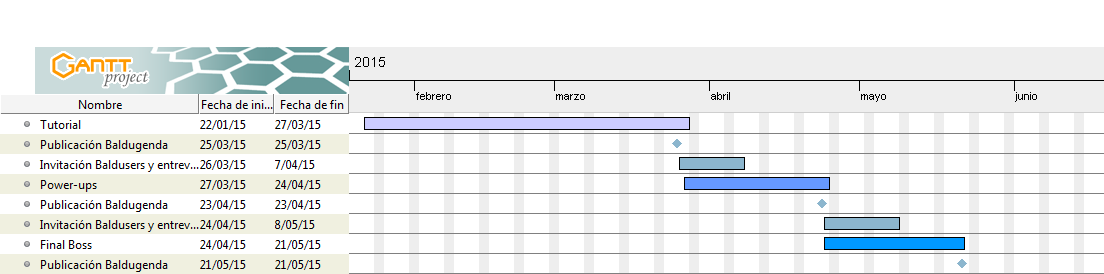
\includegraphics{figs/hitos.png}} 
    \caption{Diagrama Gantt fases de Baldugenda} 
    \label{fig:hitos} 
  \end{center} 
\end{figure}